\documentclass{article}
\usepackage{hyperref}
\usepackage[normalem]{ulem}
\usepackage{moreverb}
\usepackage{color}
\usepackage{amsmath}
\usepackage{listings}
\usepackage{graphicx}
\usepackage[top=2cm, bottom=2cm, left=2cm, right=2cm]{geometry}
\usepackage{multirow}
\usepackage{amsfonts}
\let\subsubsubsection\paragraph
\let\subsubsubsubsection\subparagraph
\lstset{breaklines=true, breakatwhitespace=true, captionpos=b, tabsize=3, showtabs=false, numbers=left, frame=single, firstnumber=1}
\usepackage[english]{babel}
\begin{document}
\tableofcontents
\begin{sloppypar}


\section{ Interest of the Tool}



\subsection{ Putting the Automata Theory Withing Reach}


\paragraph{}
Teaching abstract concepts is only possible if these concepts are put within student's reach. There are multiple ways to do this and each teacher has its own approach, as well as each student is more sensitive to some ways of knowledge transmission than to other ways. Some students might be more sensitive to the structure of the speech and the mathematical robustness of definitions, some might be more likely to assimilate knowledge if they can hear a teacher explain it, some might need to visualize concepts with their eyes, some might need a mix of several ways and the more ways are exploited to transmit things, the more student should be involved in the knowledge transmission as these ways are more complementary than redundant.

      
\paragraph{}
Teachers who are eager to maximize the number of ways they take to transmit knowledge might be interested in making abstract concepts visualizable, dynamic therefore adding a concrete aspect of the concepts. The goal of the tool is to put the automata theory in student's hands, making it manipulable (``hackable'').
      
      

\subsubsection{ Drawing automata}


\paragraph{}
One of the needed feature to automata manipulation is being able to input them in a convenient way and like others tools of the domain, the tool provides a means to input automata by drawing them with the mouse and the keyboard in a hopefully intuitive way.

         
\paragraph{}
For student who want to go farther, for repetitive tasks or big automata, the tool provides a way to write automata using a concise language instead of drawing them.

         
\paragraph{}
To display results of algorithms or automata which were written rather than drawn, the tool embeds a Javascript version\footnote{Viz.js: \href{https://github.com/mdaines/viz.js/}{https://github.com/mdaines/viz.js/}} of Graphviz\footnote{\href{http://www.graphviz.org/}{http://www.graphviz.org/}} to render graphical version of automata automatically.

         
\paragraph{}
To help writing documents about automata, the tool provides a way to export images or DOT\footnote{\href{http://www.graphviz.org/content/dot-language}{http://www.graphviz.org/content/dot-language}} codes of automata produced by the user or the tool. DOT documents can then be translated into TiKZ\footnote{\href{http://www.ctan.org/tex-archive/graphics/pgf/}{http://www.ctan.org/tex-archive/graphics/pgf/}} format in order to include automata in a LaTeX document.
      
   
      

\subsubsection{ Algorithms}


\paragraph{}
So as to let students experiment with automata-related algorithm, the tool embeds a custom programming language and some common algorithms written run algorithms (See figure \ref{aude-algo}). These algorithms are written in a dedicated language especially designed for manipulating sets and automata. 

         
\paragraph{}
The tool comes with some basic algorithms such as:
          
\begin{itemize}
	\item{ determinization: get a determinist automaton from any automaton.}
	\item{ completion: get a complete automaton from any automaton.}
	\item{ minimization: get a minimal automaton from any automaton.}
	\item{ epsilon removal: get an automaton without any epsilon transition from any automaton.}
	\item{ product: get an automaton which recognize the intersection of the two input automata's respective languages.}
	\item{ equivalence: test whether two automata recognize the same language.}
	\item{ complementation: get an automaton which recognize the complementary language of the input automaton.}
	\item{ empty and infinite language tests: test whether an automaton recognize the empty language and an infinite language, respectively}
	\item{ regular expression to automaton: get an automaton recognizing the language described by a regular expression.}
\end{itemize}
\begin{figure}[htb]\centering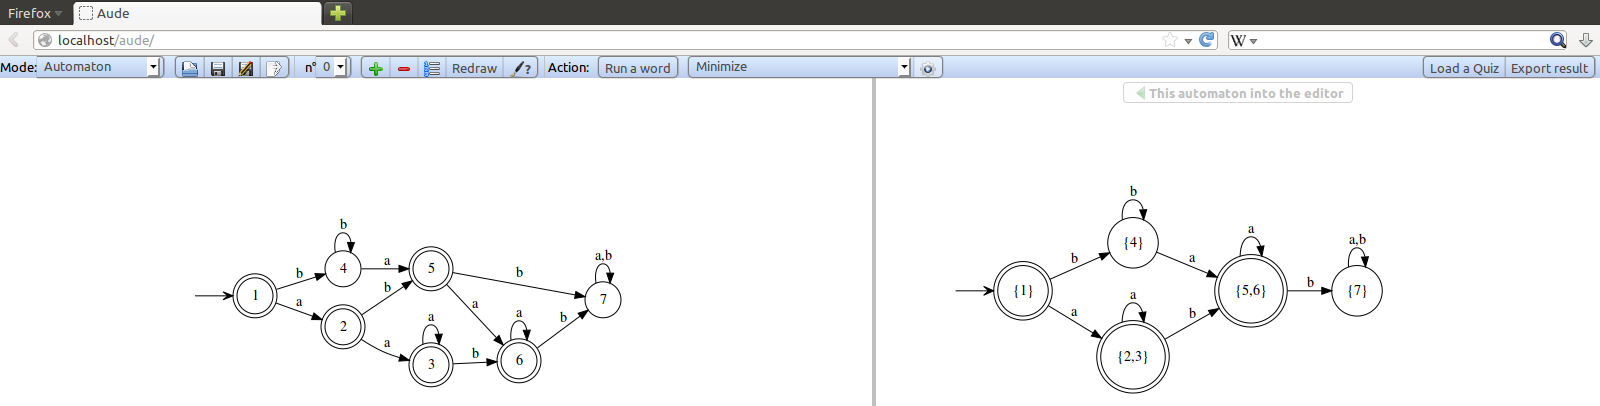
\includegraphics[width=500pt]{{../aude-algo}.png}\caption{Result of an algorithm execution.}\label{aude-algo}\end{figure}

         
\newpage
         
\paragraph{}
In addition, users can write their own algorithms using the same dedicated language as the one used for writing embedded algorithms (See figure \ref{aude-prog}).
         
          \begin{figure}[htb]\centering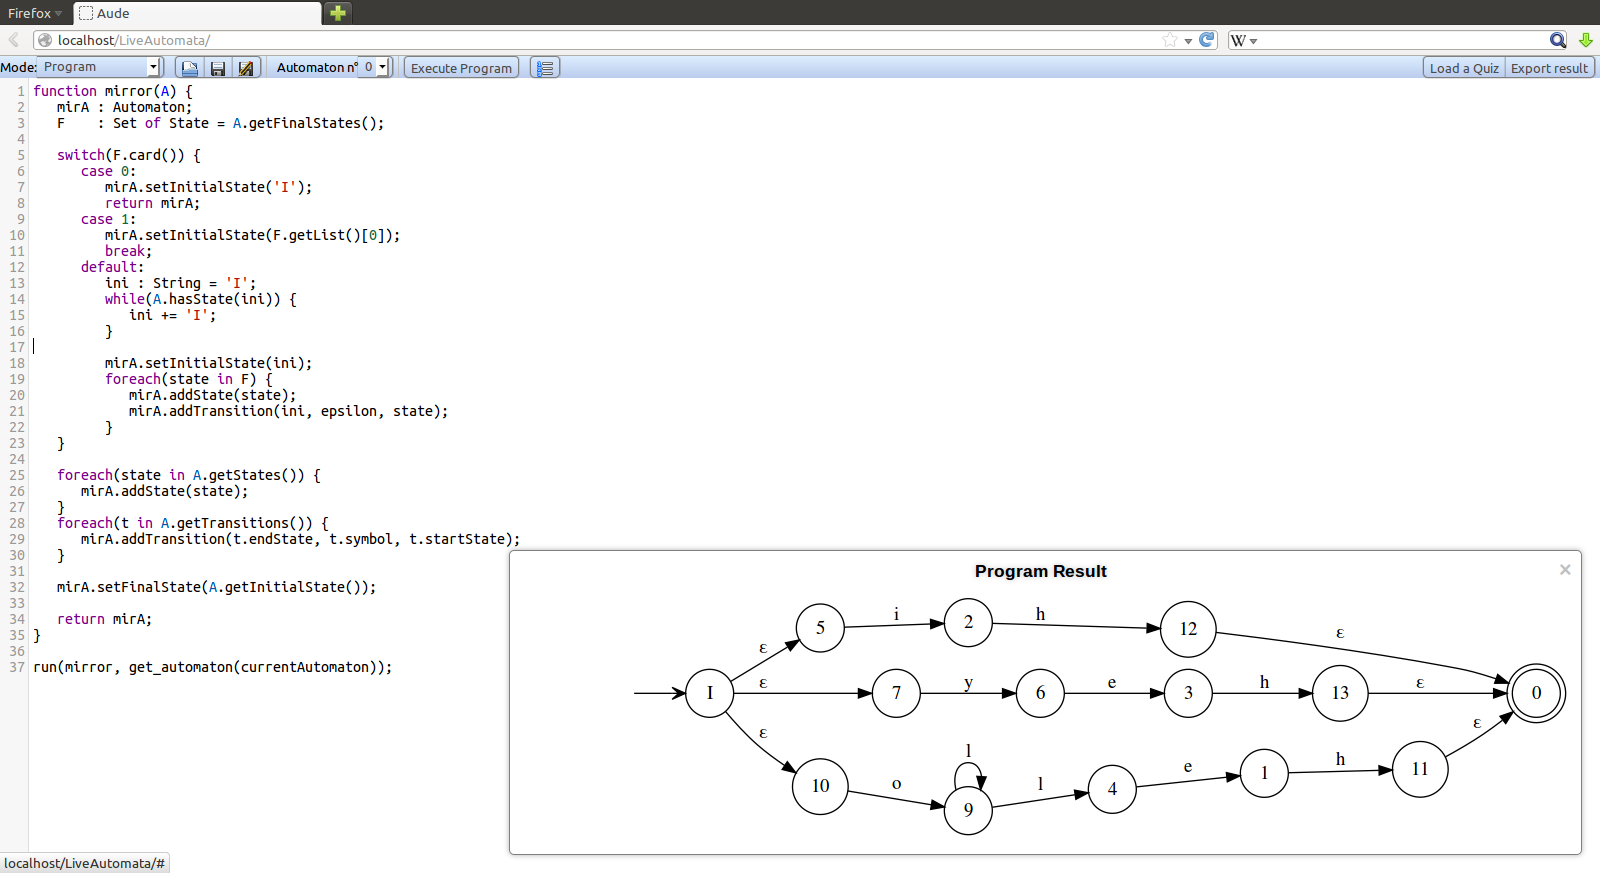
\includegraphics[width=500pt]{{../aude-prog}.png}\caption{Writing algorithms.}\label{aude-prog}\end{figure}
         
         
\paragraph{}
Algorithms can take several automata parameters. The user will be asked to choose which automata should be sent to the algorithm when running it.

          \begin{figure}[htb]\centering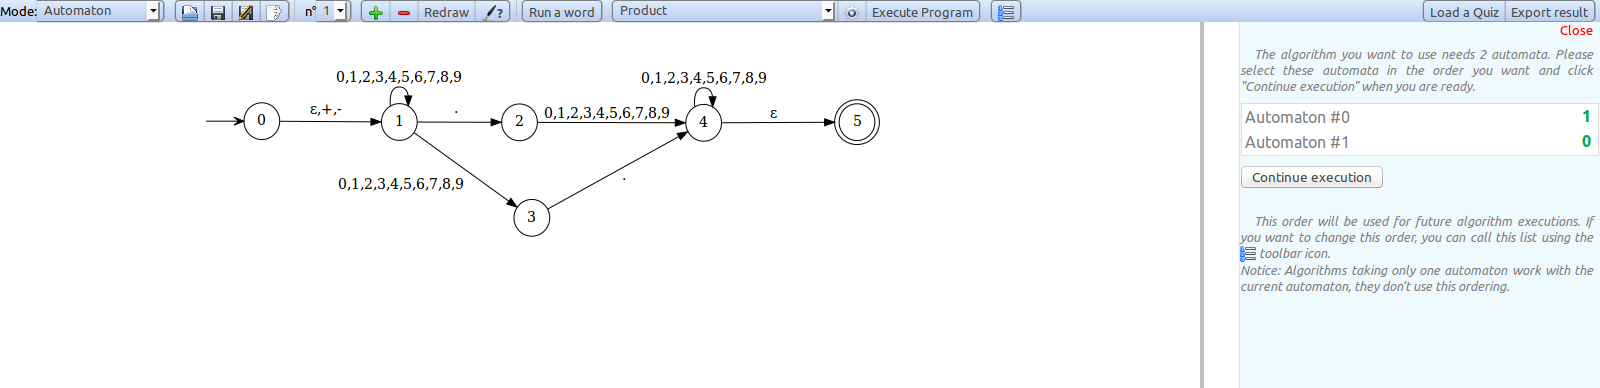
\includegraphics[width=500pt]{{../aude-list-automata}.png}\caption{Choose which automata should be sent to the algorithm.}\label{aude-list}\end{figure}
      
      

\subsubsection{ Running words}


\paragraph{}
The tool features word execution on automata. Special care was taken to make it pleasant and easy to follow by showing the execution progressively taking place, the word progressively being “consumed” (See figure \ref{word-exec}).
         
          \begin{figure}[htb]\centering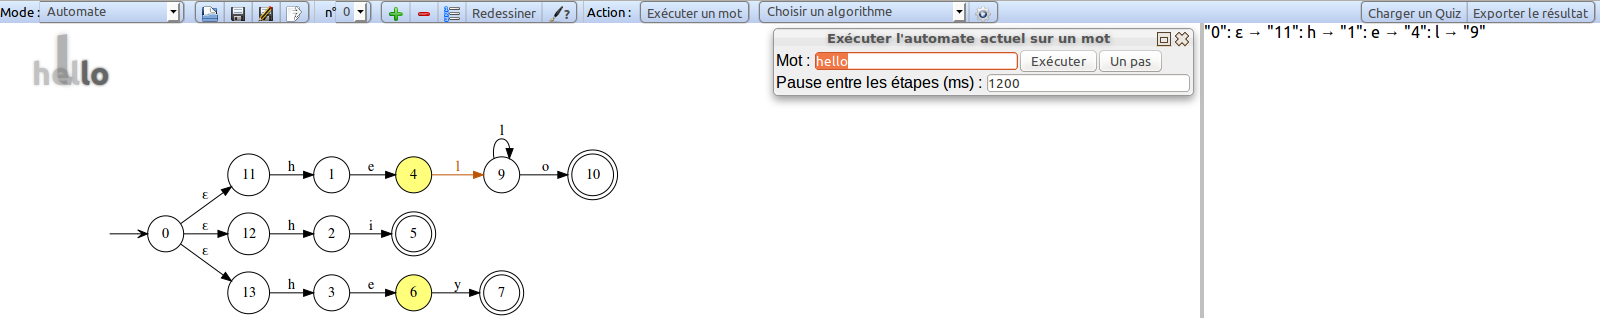
\includegraphics[width=500pt]{{../word-execution}.png}\caption{Word execution.}\label{word-exec}\end{figure}
      
      

\subsubsection{ Quiz}


\paragraph{}
With the tool, one can run custom quizzes (see picture \ref{aude-quiz}). The ability to run quizzes written by anybody (a teacher, a student) directly inside the tool, however, is probably an exclusive feature as of September 2013.

         
\paragraph{}
One can write or run quizzes featuring:
          
\begin{itemize}
	\item{ mere multiple choice questions, with zero, one or more answers, with any number of possible answers.}
	\item{ questions that ask the user to draw an automaton corresponding to a set of words.}
	\item{ questions that ask the user to draw an automaton corresponding to a language defined by an automaton or a regular expression in the quiz file.}
\end{itemize}

\paragraph{}
LaTeX can be used to write mathematics in the quiz, thanks to MathJax\footnote{\href{http://www.mathjax.org/}{http://www.mathjax.org/}}.
         
\begin{figure}[htb]\centering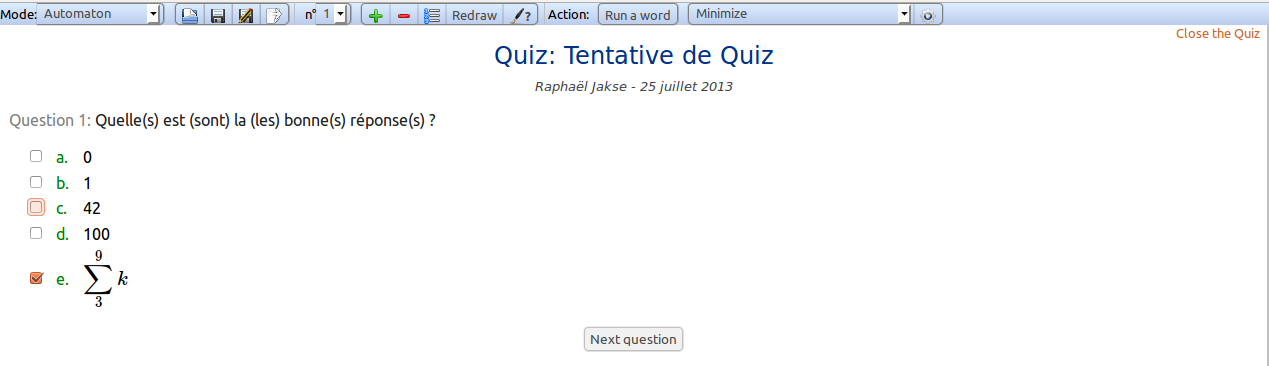
\includegraphics[width=430pt]{{../aude-quiz}.png}\caption{Quiz.}\label{aude-quiz}\end{figure}
      
   
\end{sloppypar}
\end{document}
